\section{History of Speech Synthesis}
\label{history_speech_synthesis}
Speech synthesis is not a recent ambition in history of mankind. The earliest attempts to synthesize speech are only legends starring Gerbert d'Aurillac (died 1003 A.D.), also known as Pope Sylvester II. The pretended system used by him was a brazen head: a legendary automaton imitating the anatomy of a human head and capable to answer any question. Back in those days, the brazen heads were said to be owned by wizards. Following Pope Sylvester II, some important characters in mankind history  were reputed to have one of these heads, such as Albertus Magnus or Roger Bacon \cite{butler1993myth}.

During the 18th century, Christian Kratzenstein, a German-born doctor, physicist and engineer working at the Russian Academy of Sciences, was able to built acoustics resonators similar to the human vocal tract. He activated the resonators with vibrating reeds producing the the five long vowels: /a/, /e/, /i/, /o/ and /u/ \cite{LemmettyMSc}.

Almost at the end of the 18th century, in 1791, Wolfgang von Kempelen presented his Acoustic-Mechanical Speech Machine \cite{vonKempelen}, which was able to produce single sounds and some combinations. During the first half of the 19th century, Charles Wheatstone built his improved and more complicated version of Kempelen's Acoustic-Mechanical Speech Machine, capable of producing vowels, almost all the consonants, sound combinations and even some words.	

In the late 1800's, Alexander Graham Bell also built a speaking machine and did some questionable experiments changing with his hands the vocal tract of his dog and making the dog bark in order to produce speech-like sounds \cite{Schroeder93, LemmettyMSc}.

Before World War II, Bell labs developed the vocoder, which analyzed and extracted fundamentals tone and frequency from speech. In the 1950's, the first computer based speech synthesis systems were created and in 1968 the first general English text-to-speech (TTS) system was developed at the Electrotechnical Laboratory, Japan \cite{Klatt87}. From that time on, the main branch of speech synthesis development has been focused on the investigation and development of electronic systems, but research conducted on mechanical synthesizers has not been abandoned \cite{mechSynthWeb, mechSynth}.

Speech synthesis can be defined as the artificial generation of speech. Nowadays the process has been facilitated due to the improvements made during the last 70 years in computer technology, making the computer-based speech synthesis systems lead the way supported by their flexibility and their easier access compared to mechanical systems. However, after the first resonators built by Kratzenstein, the fist speaking machine was built and presented to the world in 1791, and was obviously mechanic.

\subsection{Acoustical-Mechanical Speech Machines}
\label{history_mechanical_machines}
The speech machine developed by von Kempelen incorporated models of the lips and the tong, enabling it to produce some consonants as well as vowels. Although Kratzenstein presented his resonators before von Kempelen presented his speech machine, von Kempelen started his work quite before, publishing a book where he described the studies made on human speech production and the experiments he made with his speech machine over 20 years of work \cite{vonKempelen}.  

The machine was composed by a pressure chamber, acting as lungs, a vibrating reeds in charge of the functions of the vocal cords and a leather tube that was manually manipulated in order to change its shape as the vocal tract does in an actual person, producing different vowel sounds. It had four separate constricted passages, controlled by the fingers, to generate consonants. Von Kempelen also included in his machine a model of the vocal tract with a hinged tongue and movable lips so as to create plosive sounds \cite{Schroeder93, LemmettyMSc, flanagan_1973_speech}. 

\begin{figure}[htb]
	\begin{center}
		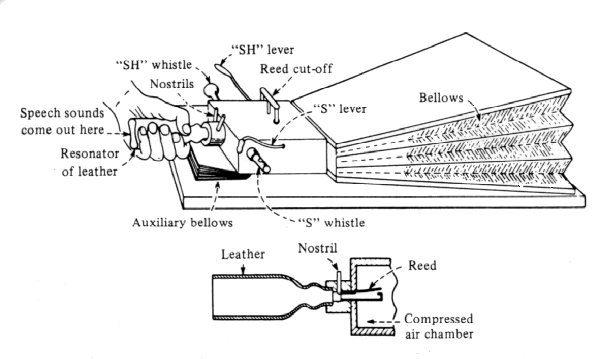
\includegraphics[width=\textwidth]{images/von_kempelen_machine.jpg}
		\caption{Reconstruction of von Kempelen's speech machine made by Wheatstone \cite{flanagan_book}}
		\label{fig:speech_machine}
	\end{center}
\end{figure}

Inspired by von Kempelen, Charles Wheatstone built an improved version of the speech machine, capable of producing vowels, consonants, some combinations and even some words. In Figure \ref{fig:speech_machine} a scheme of the machine constructed by Wheatstone is presented. Alexader Graham Bell saw the reconstruction built by Wheatstone at an exposition and, encouraged and helped by his father, made his own speaking machine, starting his way towards the contribution in the invention of the telephone.

The research with mechanical items modelling the vocal system did not give any significant improvement during the following decades, leaving the door open to alternative systems to take the lead: the electrical synthesizers with a major breakthrough: the vocoder.

\subsection{Electrical Synthesizers: The Vocoder}
\label{history_vocoder}
The first electrical device was presented to the world by Stewart in 1922 \cite{Klatt87}. It consisted of a buzzer acting as the excitation followed by two resonant circuits modelling the vocal tract. The device was able to create single static vowel sounds with two lowest formants but not any consonant nor connected sounds. A similar type of synthesizer was built by Wagner \cite{flanagan_book}, consisting on four parallel electrical resonators and excited by a buzz, capable of generating the vowel spectra when the proper combination of the outputs of the four resonators was made.

In New York's World fair 1939 \cite{flanagan_book, Klatt87, flanagan_1973_speech}, Homer Dudley presented what was consider the first full electrical synthesis device: the VODER. It was inspired by the vocoder developed at Bell Laboratoies some years earlier, which analyzed the speech into slowly varying acoustics parameters that drove the synthesizer to produce a an approximation of the speech signal. The VODER consisted of wrist bar for selecting a voicing or noise source and a foot pedal to control the fundamental frequency. The source signal was routed through ten band-pass filters controlling their output levels with the fingers \cite{LemmettyMSc}. In Figure \ref{fig:voder} the VODER structure is graphically described. As you can imagine, it was not an easy task to synthesize a sentence on this device and the speech quality and intelligibility were far from acceptable, but he demonstrated the potential to produce synthetic speech.

\begin{figure}[htb]
	\begin{center}
		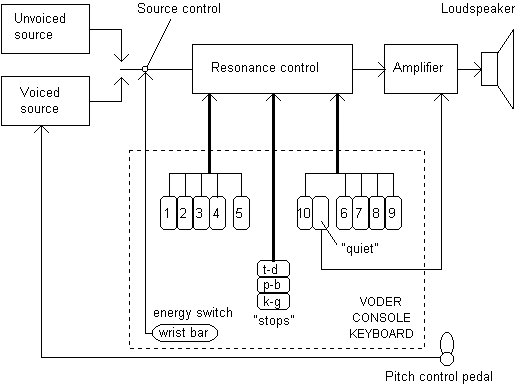
\includegraphics[width=\textwidth]{images/voder.jpg}
		\caption{VODER synthesizer \cite{Klatt87}}
		\label{fig:voder}
	\end{center}
\end{figure}

The demonstration of the VODER stimulated the scientific community and more people become interested in artificial speech generation. In 1951, Franklin Cooper lead the development of a Pattern Playback synthesizer \cite{Klatt87, flanagan_1973_speech}. The device developed at the Haskins Laboratories used optically recorded spectrogram patterns on a transparent belt to regenerate the audio signal. 

Walter Lawrence introduced in 1953 his Parametric Artificial Talker (PAT), the first formant synthesizer \cite{Klatt87}. It consisted of three parallel electronic resonators excited by a buzz or noise and a moving glass slide converted painted patterns into six different time functions to control the three formant frequencies, voicing amplitude, noise amplitude and the fundamental frequency. 

Simultaneously, the OVE I was introduced as the first cascade formant synthesizer. As its name suggest, the resonators in the OVE I were connected in cascade. A new version of this synthesizer was aired ten years later. The OVE II consisted on separate parts modelling the vocal tract to differentiate between vowels, nasals and obstruent consonants. It was excited by voicing, aspiration noise and fricative noise.

PAT and OVE developers engaged in a discussion about whether the transfer function of the acoustic tube should be modelled in parallel or in cascade. After a few years studying both systems, John Holmes presented his parallel formant synthesizer \cite{Klatt87}, obtaining a good quality in the synthesized voice.

Linear Predictive Coding (LPC) was first used in some experiments in the mid 1960's \cite{Schroeder93} and it was used in low-cost systems in 1980. The method was modified and nowadays is very useful and it can be found in many systems. 

Different TTS systems appeared during the following years. Probably, the most remarkable one was the system developed by Dennis Klatt, the Klattalk, using a new sophisticated voicing source \cite{Klatt87}, forming along MITalk, developed at the M.I.T., the basis for many systems that came after them and also many ones used nowadays \cite{LemmettyMSc}.

The modern technology used in speech synthesis involve quite sophisticated algorithms. As said in Section \ref{intro}, HMM-based systems are very popular. Actually, HMMs have been used in speech recognition for more than 30 years. In Section \ref{hmm_synthesis} a detailed description of these systems is given, as is the technique used in this project.

HMM-based systems need to extract some features or parameters from the voice, and at that point is where the vocoder comes into action. Originally, the vocoder was developed to compress the speech in telecommunication systems in order to save bandwidth by transmitting the parameters of a model in stead of the speech, as they change quite slowly compared to a speech waveform. Despite its original objective, vocoders are the interface between the audio and the speech synthesis systems, extracting the features needed to model the system and synthesizing speech from the features generated by the system. In this project we will compare two vocoders, STRAIGHT and GlottHMM. They are both described in Section \ref{vocoders}. 
